\documentclass[twoside]{book}

% Packages required by doxygen
\usepackage{fixltx2e}
\usepackage{calc}
\usepackage{doxygen}
\usepackage[export]{adjustbox} % also loads graphicx
\usepackage{graphicx}
\usepackage[utf8]{inputenc}
\usepackage{makeidx}
\usepackage{multicol}
\usepackage{multirow}
\PassOptionsToPackage{warn}{textcomp}
\usepackage{textcomp}
\usepackage[nointegrals]{wasysym}
\usepackage[table]{xcolor}

% Font selection
\usepackage[T1]{fontenc}
\usepackage[scaled=.90]{helvet}
\usepackage{courier}
\usepackage{amssymb}
\usepackage{sectsty}
\renewcommand{\familydefault}{\sfdefault}
\allsectionsfont{%
  \fontseries{bc}\selectfont%
  \color{darkgray}%
}
\renewcommand{\DoxyLabelFont}{%
  \fontseries{bc}\selectfont%
  \color{darkgray}%
}
\newcommand{\+}{\discretionary{\mbox{\scriptsize$\hookleftarrow$}}{}{}}

% Page & text layout
\usepackage{geometry}
\geometry{%
  a4paper,%
  top=2.5cm,%
  bottom=2.5cm,%
  left=2.5cm,%
  right=2.5cm%
}
\tolerance=750
\hfuzz=15pt
\hbadness=750
\setlength{\emergencystretch}{15pt}
\setlength{\parindent}{0cm}
\setlength{\parskip}{3ex plus 2ex minus 2ex}
\makeatletter
\renewcommand{\paragraph}{%
  \@startsection{paragraph}{4}{0ex}{-1.0ex}{1.0ex}{%
    \normalfont\normalsize\bfseries\SS@parafont%
  }%
}
\renewcommand{\subparagraph}{%
  \@startsection{subparagraph}{5}{0ex}{-1.0ex}{1.0ex}{%
    \normalfont\normalsize\bfseries\SS@subparafont%
  }%
}
\makeatother

% Headers & footers
\usepackage{fancyhdr}
\pagestyle{fancyplain}
\fancyhead[LE]{\fancyplain{}{\bfseries\thepage}}
\fancyhead[CE]{\fancyplain{}{}}
\fancyhead[RE]{\fancyplain{}{\bfseries\leftmark}}
\fancyhead[LO]{\fancyplain{}{\bfseries\rightmark}}
\fancyhead[CO]{\fancyplain{}{}}
\fancyhead[RO]{\fancyplain{}{\bfseries\thepage}}
\fancyfoot[LE]{\fancyplain{}{}}
\fancyfoot[CE]{\fancyplain{}{}}
\fancyfoot[RE]{\fancyplain{}{\bfseries\scriptsize Generated by Doxygen }}
\fancyfoot[LO]{\fancyplain{}{\bfseries\scriptsize Generated by Doxygen }}
\fancyfoot[CO]{\fancyplain{}{}}
\fancyfoot[RO]{\fancyplain{}{}}
\renewcommand{\footrulewidth}{0.4pt}
\renewcommand{\chaptermark}[1]{%
  \markboth{#1}{}%
}
\renewcommand{\sectionmark}[1]{%
  \markright{\thesection\ #1}%
}

% Indices & bibliography
\usepackage{natbib}
\usepackage[titles]{tocloft}
\setcounter{tocdepth}{3}
\setcounter{secnumdepth}{5}
\makeindex

% Hyperlinks (required, but should be loaded last)
\usepackage{ifpdf}
\ifpdf
  \usepackage[pdftex,pagebackref=true]{hyperref}
\else
  \usepackage[ps2pdf,pagebackref=true]{hyperref}
\fi
\hypersetup{%
  colorlinks=true,%
  linkcolor=blue,%
  citecolor=blue,%
  unicode%
}

% Custom commands
\newcommand{\clearemptydoublepage}{%
  \newpage{\pagestyle{empty}\cleardoublepage}%
}

\usepackage{caption}
\captionsetup{labelsep=space,justification=centering,font={bf},singlelinecheck=off,skip=4pt,position=top}

%===== C O N T E N T S =====

\begin{document}

% Titlepage & ToC
\hypersetup{pageanchor=false,
             bookmarksnumbered=true,
             pdfencoding=unicode
            }
\pagenumbering{roman}
\begin{titlepage}
\vspace*{7cm}
\begin{center}%
{\Large My Project }\\
\vspace*{1cm}
{\large Generated by Doxygen 1.8.11}\\
\end{center}
\end{titlepage}
\clearemptydoublepage
\tableofcontents
\clearemptydoublepage
\pagenumbering{arabic}
\hypersetup{pageanchor=true}

%--- Begin generated contents ---
\chapter{Assignment 2\+: Skeleton}
\label{index}\hypertarget{index}{}The task is to simulates the generation of data from several sensor(rangers) types, and performs data fusion.

This file should decsribe an overview of your code, what it does, what it performs, and how it should be used.

You should not simply drop the assignment specification, rather explain what will happen in your code (interface with users, and overview of logic for fusion).

Look at our other example of a dox file in week04.

~\newline
 By Alen Alempijevic ~\newline
 \href{mailto:Alen.Alempijevic@uts.edu.au}{\tt Alen.\+Alempijevic@uts.\+edu.\+au} 
\chapter{Hierarchical Index}
\section{Class Hierarchy}
This inheritance list is sorted roughly, but not completely, alphabetically\+:\begin{DoxyCompactList}
\item \contentsline{section}{Cell}{\pageref{class_cell}}{}
\item \contentsline{section}{Ranger\+:\+:data\+Sequence\+Num}{\pageref{struct_ranger_1_1data_sequence_num}}{}
\item \contentsline{section}{Ranger\+Fusion\+:\+:Point}{\pageref{struct_ranger_fusion_1_1_point}}{}
\item \contentsline{section}{Ranger\+Fusion\+Interface}{\pageref{class_ranger_fusion_interface}}{}
\begin{DoxyCompactList}
\item \contentsline{section}{Ranger\+Fusion}{\pageref{class_ranger_fusion}}{}
\end{DoxyCompactList}
\item \contentsline{section}{Ranger\+Interface}{\pageref{class_ranger_interface}}{}
\begin{DoxyCompactList}
\item \contentsline{section}{Ranger}{\pageref{class_ranger}}{}
\begin{DoxyCompactList}
\item \contentsline{section}{Laser}{\pageref{class_laser}}{}
\item \contentsline{section}{Sonar}{\pageref{class_sonar}}{}
\end{DoxyCompactList}
\end{DoxyCompactList}
\end{DoxyCompactList}

\chapter{Class Index}
\section{Class List}
Here are the classes, structs, unions and interfaces with brief descriptions\+:\begin{DoxyCompactList}
\item\contentsline{section}{\hyperlink{class_cell}{Cell} \\*Cells will be used as areas of space (rectangles) where the sensor data will be fused to indicate occupancy, default size provided, centre location draw randonly from a map of max size. On creation state is U\+N\+K\+N\+O\+WN }{\pageref{class_cell}}{}
\item\contentsline{section}{\hyperlink{struct_ranger_1_1data_sequence_num}{Ranger\+::data\+Sequence\+Num} \\*This struct can be used to keep store datasets and keep track of every sample and its sequence number.~\newline
}{\pageref{struct_ranger_1_1data_sequence_num}}{}
\item\contentsline{section}{\hyperlink{class_laser}{Laser} \\*\hyperlink{class_laser}{Laser} Shoots multiple Rangefinder rays within its field of view and returns distance readings }{\pageref{class_laser}}{}
\item\contentsline{section}{\hyperlink{struct_ranger_fusion_1_1_point}{Ranger\+Fusion\+::\+Point} \\*Can be used to store cartesian 2D co-\/ordinates~\newline
}{\pageref{struct_ranger_fusion_1_1_point}}{}
\item\contentsline{section}{\hyperlink{class_ranger}{Ranger} \\*\hyperlink{class_ranger}{Ranger} will be used as an abstract class for different type of rangefinder sensor classes }{\pageref{class_ranger}}{}
\item\contentsline{section}{\hyperlink{class_ranger_fusion}{Ranger\+Fusion} \\*\hyperlink{class_ranger_fusion}{Ranger\+Fusion} extract data from a collection of Rangers and fuses the data. }{\pageref{class_ranger_fusion}}{}
\item\contentsline{section}{\hyperlink{class_ranger_fusion_interface}{Ranger\+Fusion\+Interface} \\*Specifies the required interface for your \hyperlink{class_ranger_fusion}{Ranger\+Fusion} class your ranger fusion class must inherit from it. {\bfseries  You M\+U\+ST N\+OT edit this file } }{\pageref{class_ranger_fusion_interface}}{}
\item\contentsline{section}{\hyperlink{class_ranger_interface}{Ranger\+Interface} \\*Specifies the functionality for the \hyperlink{class_ranger}{Ranger} Class, your \hyperlink{class_ranger}{Ranger} class must inherit from it. {\bfseries  You M\+U\+ST N\+OT edit this file } }{\pageref{class_ranger_interface}}{}
\item\contentsline{section}{\hyperlink{class_sonar}{Sonar} \\*\hyperlink{class_sonar}{Sonar} Shoots one broad sonar that covers its field of view and returns maximum distance it reached }{\pageref{class_sonar}}{}
\end{DoxyCompactList}

\chapter{Class Documentation}
\hypertarget{class_cell}{}\section{Cell Class Reference}
\label{class_cell}\index{Cell@{Cell}}


Cells will be used as areas of space (rectangles) where the sensor data will be fused to indicate occupancy, default size provided, centre location draw randonly from a map of max size. On creation state is U\+N\+K\+N\+O\+WN.  




{\ttfamily \#include $<$cell.\+h$>$}

\subsection*{Public Member Functions}
\begin{DoxyCompactItemize}
\item 
\hyperlink{class_cell_a394510643e8664cf12b5efaf5cb99f71}{Cell} ()
\item 
void \hyperlink{class_cell_a9c4fd400ffbf61fe18073f3b244614ab}{set\+Side} (double side)
\item 
double \hyperlink{class_cell_a8369e6773b462215ea3c13d216621cb7}{get\+Side} (void)
\item 
double \hyperlink{class_cell_ad4fa31d97490fac2a1d11f3afaea4e67}{area} (void)
\item 
double \hyperlink{class_cell_af02495b8e758ee82478134fd491f3e13}{perimeter} (void)
\item 
void \hyperlink{class_cell_a882f75366d9cf6477d1fd7f9dd54519b}{set\+Centre} (double x, double y)
\item 
void \hyperlink{class_cell_a1087822ba50d7afea999824cca8cc1f4}{get\+Centre} (double \&x, double \&y)
\item 
cell\+::\+State \hyperlink{class_cell_aba131004c3f0bade13ef1b72e5694885}{get\+State} ()
\item 
void \hyperlink{class_cell_adeb7a033171fa07557e756f3fcc4717d}{set\+State} (cell\+::\+State)
\end{DoxyCompactItemize}


\subsection{Detailed Description}
Cells will be used as areas of space (rectangles) where the sensor data will be fused to indicate occupancy, default size provided, centre location draw randonly from a map of max size. On creation state is U\+N\+K\+N\+O\+WN. 

The \hyperlink{class_cell}{Cell} will be used for fusion accordinly\+: ~\newline
If the sensor intersects the cell and goes through \hyperlink{class_cell}{Cell} will be F\+R\+EE~\newline
If the sensor has a return from within \hyperlink{class_cell}{Cell}, it will be O\+C\+C\+U\+P\+I\+ED~\newline
 

\subsection{Constructor \& Destructor Documentation}
\index{Cell@{Cell}!Cell@{Cell}}
\index{Cell@{Cell}!Cell@{Cell}}
\subsubsection[{\texorpdfstring{Cell()}{Cell()}}]{\setlength{\rightskip}{0pt plus 5cm}Cell\+::\+Cell (
\begin{DoxyParamCaption}
{}
\end{DoxyParamCaption}
)}\hypertarget{class_cell_a394510643e8664cf12b5efaf5cb99f71}{}\label{class_cell_a394510643e8664cf12b5efaf5cb99f71}
The Default constructor sets the cell centre to values within the \#\+M\+A\+P\+\_\+\+S\+I\+ZE~\newline
\begin{DoxyNote}{Note}
N\+O\+TE\+: The cell size is also stated as \#\+D\+E\+F\+A\+U\+L\+T\+\_\+\+C\+E\+L\+L\+\_\+\+S\+I\+ZE 
\end{DoxyNote}


\subsection{Member Function Documentation}
\index{Cell@{Cell}!area@{area}}
\index{area@{area}!Cell@{Cell}}
\subsubsection[{\texorpdfstring{area(void)}{area(void)}}]{\setlength{\rightskip}{0pt plus 5cm}double Cell\+::area (
\begin{DoxyParamCaption}
\item[{void}]{}
\end{DoxyParamCaption}
)}\hypertarget{class_cell_ad4fa31d97490fac2a1d11f3afaea4e67}{}\label{class_cell_ad4fa31d97490fac2a1d11f3afaea4e67}
Member function to get area of cell \begin{DoxyReturn}{Returns}
area of cell \mbox{[}m2\mbox{]} 
\end{DoxyReturn}
\index{Cell@{Cell}!get\+Centre@{get\+Centre}}
\index{get\+Centre@{get\+Centre}!Cell@{Cell}}
\subsubsection[{\texorpdfstring{get\+Centre(double \&x, double \&y)}{getCentre(double &x, double &y)}}]{\setlength{\rightskip}{0pt plus 5cm}void Cell\+::get\+Centre (
\begin{DoxyParamCaption}
\item[{double \&}]{x, }
\item[{double \&}]{y}
\end{DoxyParamCaption}
)}\hypertarget{class_cell_a1087822ba50d7afea999824cca8cc1f4}{}\label{class_cell_a1087822ba50d7afea999824cca8cc1f4}
Member function to get centre of cell 
\begin{DoxyParams}{Parameters}
{\em x} & centre coordinate x \mbox{[}m\mbox{]} \\
\hline
{\em y} & centre coordinate y \mbox{[}m\mbox{]} \\
\hline
\end{DoxyParams}
\index{Cell@{Cell}!get\+Side@{get\+Side}}
\index{get\+Side@{get\+Side}!Cell@{Cell}}
\subsubsection[{\texorpdfstring{get\+Side(void)}{getSide(void)}}]{\setlength{\rightskip}{0pt plus 5cm}double Cell\+::get\+Side (
\begin{DoxyParamCaption}
\item[{void}]{}
\end{DoxyParamCaption}
)}\hypertarget{class_cell_a8369e6773b462215ea3c13d216621cb7}{}\label{class_cell_a8369e6773b462215ea3c13d216621cb7}
Member function to get value of the side of cell \begin{DoxyReturn}{Returns}
side of cell \mbox{[}m\mbox{]} 
\end{DoxyReturn}
\index{Cell@{Cell}!get\+State@{get\+State}}
\index{get\+State@{get\+State}!Cell@{Cell}}
\subsubsection[{\texorpdfstring{get\+State()}{getState()}}]{\setlength{\rightskip}{0pt plus 5cm}cell\+::\+State Cell\+::get\+State (
\begin{DoxyParamCaption}
{}
\end{DoxyParamCaption}
)}\hypertarget{class_cell_aba131004c3f0bade13ef1b72e5694885}{}\label{class_cell_aba131004c3f0bade13ef1b72e5694885}
Member function to get state of cell \begin{DoxyReturn}{Returns}
state of cell 
\end{DoxyReturn}
\index{Cell@{Cell}!perimeter@{perimeter}}
\index{perimeter@{perimeter}!Cell@{Cell}}
\subsubsection[{\texorpdfstring{perimeter(void)}{perimeter(void)}}]{\setlength{\rightskip}{0pt plus 5cm}double Cell\+::perimeter (
\begin{DoxyParamCaption}
\item[{void}]{}
\end{DoxyParamCaption}
)}\hypertarget{class_cell_af02495b8e758ee82478134fd491f3e13}{}\label{class_cell_af02495b8e758ee82478134fd491f3e13}
Member function to get perimeter of cell \begin{DoxyReturn}{Returns}
perimieter of cell \mbox{[}m\mbox{]} 
\end{DoxyReturn}
\index{Cell@{Cell}!set\+Centre@{set\+Centre}}
\index{set\+Centre@{set\+Centre}!Cell@{Cell}}
\subsubsection[{\texorpdfstring{set\+Centre(double x, double y)}{setCentre(double x, double y)}}]{\setlength{\rightskip}{0pt plus 5cm}void Cell\+::set\+Centre (
\begin{DoxyParamCaption}
\item[{double}]{x, }
\item[{double}]{y}
\end{DoxyParamCaption}
)}\hypertarget{class_cell_a882f75366d9cf6477d1fd7f9dd54519b}{}\label{class_cell_a882f75366d9cf6477d1fd7f9dd54519b}
Member function to set centre of cell 
\begin{DoxyParams}{Parameters}
{\em x} & centre coordinate x \mbox{[}m\mbox{]} \\
\hline
{\em y} & centre coordinate y \mbox{[}m\mbox{]} \\
\hline
\end{DoxyParams}
\index{Cell@{Cell}!set\+Side@{set\+Side}}
\index{set\+Side@{set\+Side}!Cell@{Cell}}
\subsubsection[{\texorpdfstring{set\+Side(double side)}{setSide(double side)}}]{\setlength{\rightskip}{0pt plus 5cm}void Cell\+::set\+Side (
\begin{DoxyParamCaption}
\item[{double}]{side}
\end{DoxyParamCaption}
)}\hypertarget{class_cell_a9c4fd400ffbf61fe18073f3b244614ab}{}\label{class_cell_a9c4fd400ffbf61fe18073f3b244614ab}
Member function sets Side 
\begin{DoxyParams}{Parameters}
{\em side} & The desired side length \\
\hline
\end{DoxyParams}
\index{Cell@{Cell}!set\+State@{set\+State}}
\index{set\+State@{set\+State}!Cell@{Cell}}
\subsubsection[{\texorpdfstring{set\+State(cell\+::\+State)}{setState(cell::State)}}]{\setlength{\rightskip}{0pt plus 5cm}void Cell\+::set\+State (
\begin{DoxyParamCaption}
\item[{cell\+::\+State}]{state}
\end{DoxyParamCaption}
)}\hypertarget{class_cell_adeb7a033171fa07557e756f3fcc4717d}{}\label{class_cell_adeb7a033171fa07557e756f3fcc4717d}
Member function to set state of cell 
\begin{DoxyParams}{Parameters}
{\em area} & of cell \\
\hline
\end{DoxyParams}


The documentation for this class was generated from the following files\+:\begin{DoxyCompactItemize}
\item 
cell.\+h\item 
cell.\+cpp\end{DoxyCompactItemize}

\hypertarget{struct_ranger_1_1data_sequence_num}{}\section{Ranger\+:\+:data\+Sequence\+Num Struct Reference}
\label{struct_ranger_1_1data_sequence_num}\index{Ranger\+::data\+Sequence\+Num@{Ranger\+::data\+Sequence\+Num}}


This struct can be used to keep store datasets and keep track of every sample and its sequence number.~\newline
.  




{\ttfamily \#include $<$ranger.\+h$>$}

\subsection*{Public Attributes}
\begin{DoxyCompactItemize}
\item 
unsigned int {\bfseries sample\+No}\hypertarget{struct_ranger_1_1data_sequence_num_a445b538f2723e28ecd491e7134aebf2a}{}\label{struct_ranger_1_1data_sequence_num_a445b538f2723e28ecd491e7134aebf2a}

\item 
std\+::vector$<$ double $>$ {\bfseries data}\hypertarget{struct_ranger_1_1data_sequence_num_ae830d296270962774b3958c2ab3e7e4d}{}\label{struct_ranger_1_1data_sequence_num_ae830d296270962774b3958c2ab3e7e4d}

\end{DoxyCompactItemize}


\subsection{Detailed Description}
This struct can be used to keep store datasets and keep track of every sample and its sequence number.~\newline
. 

The struct consists of following elements\+:~\newline

\begin{DoxyItemize}
\item Sample Number(unsigned int)~\newline

\item Dataset of the sample (A vector of double)~\newline

\end{DoxyItemize}

The documentation for this struct was generated from the following file\+:\begin{DoxyCompactItemize}
\item 
ranger.\+h\end{DoxyCompactItemize}

\hypertarget{class_laser}{}\section{Laser Class Reference}
\label{class_laser}\index{Laser@{Laser}}


\hyperlink{class_laser}{Laser} Shoots multiple Rangefinder rays within its field of view and returns distance readings.  




{\ttfamily \#include $<$laser.\+h$>$}



Inheritance diagram for Laser\+:
\nopagebreak
\begin{figure}[H]
\begin{center}
\leavevmode
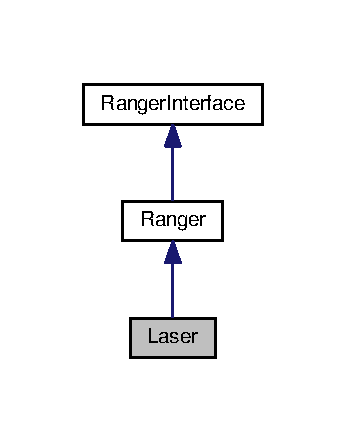
\includegraphics[width=166pt]{class_laser__inherit__graph}
\end{center}
\end{figure}


Collaboration diagram for Laser\+:
\nopagebreak
\begin{figure}[H]
\begin{center}
\leavevmode
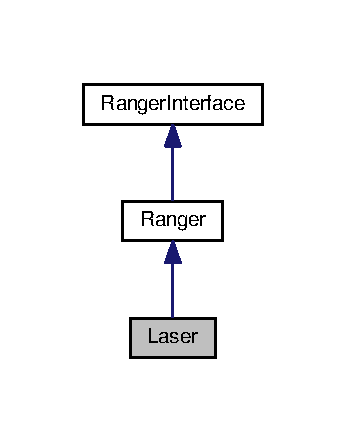
\includegraphics[width=166pt]{class_laser__coll__graph}
\end{center}
\end{figure}
\subsection*{Public Member Functions}
\begin{DoxyCompactItemize}
\item 
\hyperlink{class_laser_a68465e89283dffcc29a37e94693c6f87}{Laser} ()
\item 
bool \hyperlink{class_laser_a5f140784aae7e82c2aa0f690548d6ebb}{set\+Field\+Of\+View} (unsigned int fov)
\item 
std\+::vector$<$ double $>$ \hyperlink{class_laser_af2d93a5e123f3b637be6d3383019562b}{generate\+Data} ()
\begin{DoxyCompactList}\small\item\em This function generates random range readings as data using supplied random number generator~\newline
using normal distribution with mean of 4m and standard deviation of 5m. \end{DoxyCompactList}\item 
\hyperlink{struct_ranger_1_1data_sequence_num}{data\+Sequence\+Num} \hyperlink{class_laser_a35d376014dcf81c217e8bbe1bfd34926}{query\+Sample} (unsigned int \&a)
\end{DoxyCompactItemize}
\subsection*{Additional Inherited Members}


\subsection{Detailed Description}
\hyperlink{class_laser}{Laser} Shoots multiple Rangefinder rays within its field of view and returns distance readings. 

The \hyperlink{class_laser}{Laser} works accordingly\+: ~\newline
It shoots multiple number of laser within its field of view.~\newline
Number of \hyperlink{class_laser}{Laser} rays depends on field of view and Angular Resolution ~\newline
Then it returns the distances of the nearest obstructions each \hyperlink{class_laser}{Laser} hits.~\newline
 

\subsection{Constructor \& Destructor Documentation}
\index{Laser@{Laser}!Laser@{Laser}}
\index{Laser@{Laser}!Laser@{Laser}}
\subsubsection[{\texorpdfstring{Laser()}{Laser()}}]{\setlength{\rightskip}{0pt plus 5cm}Laser\+::\+Laser (
\begin{DoxyParamCaption}
{}
\end{DoxyParamCaption}
)}\hypertarget{class_laser_a68465e89283dffcc29a37e94693c6f87}{}\label{class_laser_a68465e89283dffcc29a37e94693c6f87}
Default constructor -\/ all sensor attributes set to a default values for \hyperlink{class_laser}{Laser} 

\subsection{Member Function Documentation}
\index{Laser@{Laser}!generate\+Data@{generate\+Data}}
\index{generate\+Data@{generate\+Data}!Laser@{Laser}}
\subsubsection[{\texorpdfstring{generate\+Data()}{generateData()}}]{\setlength{\rightskip}{0pt plus 5cm}std\+::vector$<$ double $>$ Laser\+::generate\+Data (
\begin{DoxyParamCaption}
{}
\end{DoxyParamCaption}
)\hspace{0.3cm}{\ttfamily [virtual]}}\hypertarget{class_laser_af2d93a5e123f3b637be6d3383019562b}{}\label{class_laser_af2d93a5e123f3b637be6d3383019562b}


This function generates random range readings as data using supplied random number generator~\newline
using normal distribution with mean of 4m and standard deviation of 5m. 

Member function to genarate \hyperlink{class_laser}{Laser} Readings \begin{DoxyReturn}{Returns}
dataset of range readings\mbox{[}m\mbox{]} 
\end{DoxyReturn}


Implements \hyperlink{class_ranger_a1ac4a84f251b0793fc262643080f084a}{Ranger}.

\index{Laser@{Laser}!query\+Sample@{query\+Sample}}
\index{query\+Sample@{query\+Sample}!Laser@{Laser}}
\subsubsection[{\texorpdfstring{query\+Sample(unsigned int \&a)}{querySample(unsigned int &a)}}]{\setlength{\rightskip}{0pt plus 5cm}{\bf Laser\+::data\+Sequence\+Num} Laser\+::query\+Sample (
\begin{DoxyParamCaption}
\item[{unsigned int \&}]{a}
\end{DoxyParamCaption}
)\hspace{0.3cm}{\ttfamily [virtual]}}\hypertarget{class_laser_a35d376014dcf81c217e8bbe1bfd34926}{}\label{class_laser_a35d376014dcf81c217e8bbe1bfd34926}
Member function that can be used to query stored datasets of \hyperlink{class_laser}{Laser} 
\begin{DoxyParams}{Parameters}
{\em Desired} & Sample Number \\
\hline
\end{DoxyParams}
\begin{DoxyReturn}{Returns}
a struct that consists of\+: ~\newline

\begin{DoxyItemize}
\item Sample Number~\newline

\item Dataset\mbox{[}m\mbox{]} 
\end{DoxyItemize}
\end{DoxyReturn}


Implements \hyperlink{class_ranger_adbde91455d069a471c890e2aa808c0d3}{Ranger}.

\index{Laser@{Laser}!set\+Field\+Of\+View@{set\+Field\+Of\+View}}
\index{set\+Field\+Of\+View@{set\+Field\+Of\+View}!Laser@{Laser}}
\subsubsection[{\texorpdfstring{set\+Field\+Of\+View(unsigned int fov)}{setFieldOfView(unsigned int fov)}}]{\setlength{\rightskip}{0pt plus 5cm}bool Laser\+::set\+Field\+Of\+View (
\begin{DoxyParamCaption}
\item[{unsigned int}]{fov}
\end{DoxyParamCaption}
)\hspace{0.3cm}{\ttfamily [virtual]}}\hypertarget{class_laser_a5f140784aae7e82c2aa0f690548d6ebb}{}\label{class_laser_a5f140784aae7e82c2aa0f690548d6ebb}
Member function sets Field of View 
\begin{DoxyParams}{Parameters}
{\em Desired} & Field of View \\
\hline
\end{DoxyParams}
\begin{DoxyReturn}{Returns}
a boolean indicating if passed value is compatible with \hyperlink{class_laser}{Laser}. 
\end{DoxyReturn}


Implements \hyperlink{class_ranger_a9cebe84c1aec338dc0b72baff48ea9d4}{Ranger}.



The documentation for this class was generated from the following files\+:\begin{DoxyCompactItemize}
\item 
laser.\+h\item 
laser.\+cpp\end{DoxyCompactItemize}

\hypertarget{struct_ranger_fusion_1_1_point}{}\section{Ranger\+Fusion\+:\+:Point Struct Reference}
\label{struct_ranger_fusion_1_1_point}\index{Ranger\+Fusion\+::\+Point@{Ranger\+Fusion\+::\+Point}}


Can be used to store cartesian 2D co-\/ordinates~\newline
.  




{\ttfamily \#include $<$rangerfusion.\+h$>$}

\subsection*{Public Attributes}
\begin{DoxyCompactItemize}
\item 
double {\bfseries x}\hypertarget{struct_ranger_fusion_1_1_point_aad4a1484b0897795f2cf1c425054439a}{}\label{struct_ranger_fusion_1_1_point_aad4a1484b0897795f2cf1c425054439a}

\item 
double {\bfseries y}\hypertarget{struct_ranger_fusion_1_1_point_a7684058bf1b973f45620ab211bf1c4eb}{}\label{struct_ranger_fusion_1_1_point_a7684058bf1b973f45620ab211bf1c4eb}

\end{DoxyCompactItemize}


\subsection{Detailed Description}
Can be used to store cartesian 2D co-\/ordinates~\newline
. 

The struct consists of following elements\+:~\newline

\begin{DoxyItemize}
\item Position in reference to X axis(double)~\newline

\item Position in reference to X axis(double)~\newline

\end{DoxyItemize}

The documentation for this struct was generated from the following file\+:\begin{DoxyCompactItemize}
\item 
rangerfusion.\+h\end{DoxyCompactItemize}

\hypertarget{class_ranger}{}\section{Ranger Class Reference}
\label{class_ranger}\index{Ranger@{Ranger}}


\hyperlink{class_ranger}{Ranger} will be used as an abstract class for different type of rangefinder sensor classes .  




{\ttfamily \#include $<$ranger.\+h$>$}



Inheritance diagram for Ranger\+:
\nopagebreak
\begin{figure}[H]
\begin{center}
\leavevmode
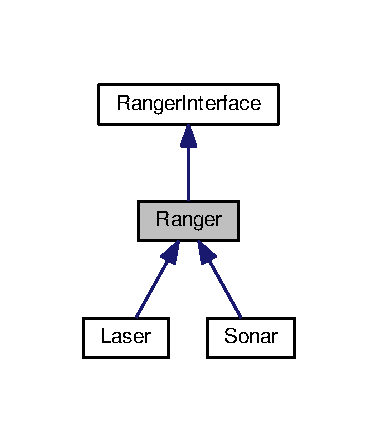
\includegraphics[width=182pt]{class_ranger__inherit__graph}
\end{center}
\end{figure}


Collaboration diagram for Ranger\+:
\nopagebreak
\begin{figure}[H]
\begin{center}
\leavevmode
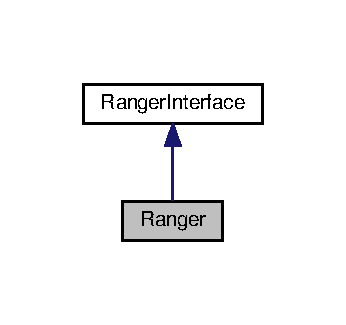
\includegraphics[width=166pt]{class_ranger__coll__graph}
\end{center}
\end{figure}
\subsection*{Classes}
\begin{DoxyCompactItemize}
\item 
struct \hyperlink{struct_ranger_1_1data_sequence_num}{data\+Sequence\+Num}
\begin{DoxyCompactList}\small\item\em This struct can be used to keep store datasets and keep track of every sample and its sequence number.~\newline
. \end{DoxyCompactList}\end{DoxyCompactItemize}
\subsection*{Public Member Functions}
\begin{DoxyCompactItemize}
\item 
\hyperlink{class_ranger_a65e1b9530f370b95cd673690c5bf02b5}{Ranger} ()
\item 
unsigned int \hyperlink{class_ranger_a95b5013ae191d1e19b93fab002306718}{get\+Angular\+Resolution} (void)
\item 
int \hyperlink{class_ranger_a1952b96d8dcbeb6afa107c8453d778a5}{get\+Angular\+Offset} (void)
\item 
unsigned int \hyperlink{class_ranger_a4bca7dce56b7959257d90b1f30bf0271}{get\+Field\+Of\+View} (void)
\item 
double \hyperlink{class_ranger_aba5e81260e55089d9ff869051156a722}{get\+Max\+Range} (void)
\item 
double \hyperlink{class_ranger_a646a06d3916179b9ebc4502bad169eec}{get\+Min\+Range} (void)
\item 
ranger\+::\+Sensing\+Method \hyperlink{class_ranger_a47e30b7ec55adec5bb542278ccfee140}{get\+Sensing\+Method} (void)
\item 
std\+::string \hyperlink{class_ranger_a00c1e787c323b1e1aa28333059fc4db5}{get\+Model} (void)
\item 
unsigned int \hyperlink{class_ranger_aff4dcbd8b1c63edfba7b474176860627}{get\+Sequence\+No} (void)
\item 
bool \hyperlink{class_ranger_a3dc62dcba54eefbd7a0f08cbf97d87dc}{set\+Angular\+Resolution} (unsigned int resolution)
\item 
bool \hyperlink{class_ranger_ae1b15546cf48d942f86ea1031e9be486}{set\+Angular\+Offset} (int offset)
\item 
virtual bool \hyperlink{class_ranger_a9cebe84c1aec338dc0b72baff48ea9d4}{set\+Field\+Of\+View} (unsigned int fov)=0
\item 
virtual std\+::vector$<$ double $>$ \hyperlink{class_ranger_a1ac4a84f251b0793fc262643080f084a}{generate\+Data} ()=0
\begin{DoxyCompactList}\small\item\em This function should be implimented in the inherited child class to generate data~\newline
 using seeded random number generator supplied from ranger class. \end{DoxyCompactList}\item 
virtual \hyperlink{struct_ranger_1_1data_sequence_num}{data\+Sequence\+Num} \hyperlink{class_ranger_adbde91455d069a471c890e2aa808c0d3}{query\+Sample} (unsigned int \&a)=0
\end{DoxyCompactItemize}
\subsection*{Protected Attributes}
\begin{DoxyCompactItemize}
\item 
unsigned int {\bfseries angular\+Reso\+\_\+}\hypertarget{class_ranger_a53534cf242b7da6e4766016c24876d55}{}\label{class_ranger_a53534cf242b7da6e4766016c24876d55}

\item 
unsigned int \hyperlink{class_ranger_a013937201e2a4a516d4d36cac0193d68}{fov\+\_\+}\hypertarget{class_ranger_a013937201e2a4a516d4d36cac0193d68}{}\label{class_ranger_a013937201e2a4a516d4d36cac0193d68}

\begin{DoxyCompactList}\small\item\em Angular Resolution and Field of View of \hyperlink{class_ranger}{Ranger}. \end{DoxyCompactList}\item 
int \hyperlink{class_ranger_add17fe15ea0db50db1f678f9949cfc87}{offset\+\_\+}\hypertarget{class_ranger_add17fe15ea0db50db1f678f9949cfc87}{}\label{class_ranger_add17fe15ea0db50db1f678f9949cfc87}

\begin{DoxyCompactList}\small\item\em Angular Offset of \hyperlink{class_ranger}{Ranger}. \end{DoxyCompactList}\item 
double {\bfseries min\+Range\+\_\+}\hypertarget{class_ranger_a3dddeb9eb109baf567dfcd356706c6fb}{}\label{class_ranger_a3dddeb9eb109baf567dfcd356706c6fb}

\item 
double \hyperlink{class_ranger_aa92901df85f1818f27c0cf2e56ac2667}{max\+Range\+\_\+}\hypertarget{class_ranger_aa92901df85f1818f27c0cf2e56ac2667}{}\label{class_ranger_aa92901df85f1818f27c0cf2e56ac2667}

\begin{DoxyCompactList}\small\item\em Minimum and Maximum Range Capacity of the Sensor. \end{DoxyCompactList}\item 
unsigned int \hyperlink{class_ranger_a19d2d3776438ff0fe7060d3fcdc46111}{num\+Of\+Samples}\hypertarget{class_ranger_a19d2d3776438ff0fe7060d3fcdc46111}{}\label{class_ranger_a19d2d3776438ff0fe7060d3fcdc46111}

\begin{DoxyCompactList}\small\item\em Number of sensor reading extracted in Samples. \end{DoxyCompactList}\item 
unsigned int \hyperlink{class_ranger_a3d56c77b50d945e89809cae1a93d0046}{seed}\hypertarget{class_ranger_a3d56c77b50d945e89809cae1a93d0046}{}\label{class_ranger_a3d56c77b50d945e89809cae1a93d0046}

\begin{DoxyCompactList}\small\item\em seed for Random Number generator \end{DoxyCompactList}\item 
std\+::default\+\_\+random\+\_\+engine \hyperlink{class_ranger_aa8678414feb7c07f6aee40d889619064}{generator}\hypertarget{class_ranger_aa8678414feb7c07f6aee40d889619064}{}\label{class_ranger_aa8678414feb7c07f6aee40d889619064}

\begin{DoxyCompactList}\small\item\em Random Number generator to supply random sensor readings. \end{DoxyCompactList}\item 
ranger\+::\+Sensing\+Method \hyperlink{class_ranger_a59c4423a891952a753560b2dc79aa3c5}{sensing\+Type\+\_\+}\hypertarget{class_ranger_a59c4423a891952a753560b2dc79aa3c5}{}\label{class_ranger_a59c4423a891952a753560b2dc79aa3c5}

\begin{DoxyCompactList}\small\item\em Specific Sensing Type of the \hyperlink{class_ranger}{Ranger}. \end{DoxyCompactList}\item 
std\+::vector$<$ double $>$ \hyperlink{class_ranger_adef7fed47f032646f5023046de0bbc48}{data\+\_\+}\hypertarget{class_ranger_adef7fed47f032646f5023046de0bbc48}{}\label{class_ranger_adef7fed47f032646f5023046de0bbc48}

\begin{DoxyCompactList}\small\item\em Container to store data for each execution. \end{DoxyCompactList}\item 
std\+::string \hyperlink{class_ranger_a806db893039467e1f6f66335e8eabb7b}{model\+\_\+}\hypertarget{class_ranger_a806db893039467e1f6f66335e8eabb7b}{}\label{class_ranger_a806db893039467e1f6f66335e8eabb7b}

\begin{DoxyCompactList}\small\item\em Model Name of the \hyperlink{class_ranger}{Ranger}. \end{DoxyCompactList}\item 
unsigned int \hyperlink{class_ranger_a8bb86299b941e0e0b38c958f214641ea}{sequence\+No}\hypertarget{class_ranger_a8bb86299b941e0e0b38c958f214641ea}{}\label{class_ranger_a8bb86299b941e0e0b38c958f214641ea}

\begin{DoxyCompactList}\small\item\em Sequence Number of generated data. \end{DoxyCompactList}\end{DoxyCompactItemize}


\subsection{Detailed Description}
\hyperlink{class_ranger}{Ranger} will be used as an abstract class for different type of rangefinder sensor classes . 

this class consists of basic features of a rangefinder sensor which includes\+:~\newline
Orientation Offset, Field of View, Angular Resolution, Number of Samples, Sensing Type, Data~\newline
classes inherited from this class can conduct computations by adding functions for the features that are exclusiveto them~\newline
 

\subsection{Constructor \& Destructor Documentation}
\index{Ranger@{Ranger}!Ranger@{Ranger}}
\index{Ranger@{Ranger}!Ranger@{Ranger}}
\subsubsection[{\texorpdfstring{Ranger()}{Ranger()}}]{\setlength{\rightskip}{0pt plus 5cm}Ranger\+::\+Ranger (
\begin{DoxyParamCaption}
{}
\end{DoxyParamCaption}
)}\hypertarget{class_ranger_a65e1b9530f370b95cd673690c5bf02b5}{}\label{class_ranger_a65e1b9530f370b95cd673690c5bf02b5}
The Default constructor sets all the attributes to zero. Inherited Child classes are suppose to configure these Parameters~\newline
Besides it initiates a seed and a random number generator which can be used by child classes to generate data .~\newline
\begin{DoxyNote}{Note}
N\+O\+TE\+: All the member variables should be set to default values in child classes 
\end{DoxyNote}


\subsection{Member Function Documentation}
\index{Ranger@{Ranger}!generate\+Data@{generate\+Data}}
\index{generate\+Data@{generate\+Data}!Ranger@{Ranger}}
\subsubsection[{\texorpdfstring{generate\+Data()=0}{generateData()=0}}]{\setlength{\rightskip}{0pt plus 5cm}virtual std\+::vector$<$double$>$ Ranger\+::generate\+Data (
\begin{DoxyParamCaption}
{}
\end{DoxyParamCaption}
)\hspace{0.3cm}{\ttfamily [pure virtual]}}\hypertarget{class_ranger_a1ac4a84f251b0793fc262643080f084a}{}\label{class_ranger_a1ac4a84f251b0793fc262643080f084a}


This function should be implimented in the inherited child class to generate data~\newline
 using seeded random number generator supplied from ranger class. 

Pure Virtual function generates data \begin{DoxyReturn}{Returns}
dataset of range readings\mbox{[}m\mbox{]} 
\end{DoxyReturn}


Implements \hyperlink{class_ranger_interface}{Ranger\+Interface}.



Implemented in \hyperlink{class_laser_af2d93a5e123f3b637be6d3383019562b}{Laser}, and \hyperlink{class_sonar_a33cc5f2df6cc1d96a59067be67eab781}{Sonar}.

\index{Ranger@{Ranger}!get\+Angular\+Offset@{get\+Angular\+Offset}}
\index{get\+Angular\+Offset@{get\+Angular\+Offset}!Ranger@{Ranger}}
\subsubsection[{\texorpdfstring{get\+Angular\+Offset(void)}{getAngularOffset(void)}}]{\setlength{\rightskip}{0pt plus 5cm}int Ranger\+::get\+Angular\+Offset (
\begin{DoxyParamCaption}
\item[{void}]{}
\end{DoxyParamCaption}
)\hspace{0.3cm}{\ttfamily [virtual]}}\hypertarget{class_ranger_a1952b96d8dcbeb6afa107c8453d778a5}{}\label{class_ranger_a1952b96d8dcbeb6afa107c8453d778a5}
Member function to get angle of offset from the Y axis \begin{DoxyReturn}{Returns}
Angle Offset of \hyperlink{class_ranger}{Ranger} \mbox{[}Degree\mbox{]} 
\end{DoxyReturn}


Implements \hyperlink{class_ranger_interface_a3af867912dfc4f2cf899f53b82e85130}{Ranger\+Interface}.

\index{Ranger@{Ranger}!get\+Angular\+Resolution@{get\+Angular\+Resolution}}
\index{get\+Angular\+Resolution@{get\+Angular\+Resolution}!Ranger@{Ranger}}
\subsubsection[{\texorpdfstring{get\+Angular\+Resolution(void)}{getAngularResolution(void)}}]{\setlength{\rightskip}{0pt plus 5cm}unsigned int Ranger\+::get\+Angular\+Resolution (
\begin{DoxyParamCaption}
\item[{void}]{}
\end{DoxyParamCaption}
)\hspace{0.3cm}{\ttfamily [virtual]}}\hypertarget{class_ranger_a95b5013ae191d1e19b93fab002306718}{}\label{class_ranger_a95b5013ae191d1e19b93fab002306718}
Member function to get Angular Resolution of the ranger \begin{DoxyReturn}{Returns}
Angular Resolution of \hyperlink{class_ranger}{Ranger} \mbox{[}Degree\mbox{]} 
\end{DoxyReturn}


Implements \hyperlink{class_ranger_interface_a37d4f89daffa8b2708dfc11034893552}{Ranger\+Interface}.

\index{Ranger@{Ranger}!get\+Field\+Of\+View@{get\+Field\+Of\+View}}
\index{get\+Field\+Of\+View@{get\+Field\+Of\+View}!Ranger@{Ranger}}
\subsubsection[{\texorpdfstring{get\+Field\+Of\+View(void)}{getFieldOfView(void)}}]{\setlength{\rightskip}{0pt plus 5cm}unsigned int Ranger\+::get\+Field\+Of\+View (
\begin{DoxyParamCaption}
\item[{void}]{}
\end{DoxyParamCaption}
)\hspace{0.3cm}{\ttfamily [virtual]}}\hypertarget{class_ranger_a4bca7dce56b7959257d90b1f30bf0271}{}\label{class_ranger_a4bca7dce56b7959257d90b1f30bf0271}
Member function to get angle of Field of View of \hyperlink{class_ranger}{Ranger}. \begin{DoxyReturn}{Returns}
Field of View of \hyperlink{class_ranger}{Ranger} \mbox{[}Degree\mbox{]} 
\end{DoxyReturn}


Implements \hyperlink{class_ranger_interface_a18716da6932402b8dda75f682be6f06c}{Ranger\+Interface}.

\index{Ranger@{Ranger}!get\+Max\+Range@{get\+Max\+Range}}
\index{get\+Max\+Range@{get\+Max\+Range}!Ranger@{Ranger}}
\subsubsection[{\texorpdfstring{get\+Max\+Range(void)}{getMaxRange(void)}}]{\setlength{\rightskip}{0pt plus 5cm}double Ranger\+::get\+Max\+Range (
\begin{DoxyParamCaption}
\item[{void}]{}
\end{DoxyParamCaption}
)\hspace{0.3cm}{\ttfamily [virtual]}}\hypertarget{class_ranger_aba5e81260e55089d9ff869051156a722}{}\label{class_ranger_aba5e81260e55089d9ff869051156a722}
Member function to get value possible Maximum Range of Sensor \begin{DoxyReturn}{Returns}
Maximum Range of \hyperlink{class_ranger}{Ranger} \mbox{[}m\mbox{]} 
\end{DoxyReturn}


Implements \hyperlink{class_ranger_interface_a0bb29a41de5767c99081002c0590c186}{Ranger\+Interface}.

\index{Ranger@{Ranger}!get\+Min\+Range@{get\+Min\+Range}}
\index{get\+Min\+Range@{get\+Min\+Range}!Ranger@{Ranger}}
\subsubsection[{\texorpdfstring{get\+Min\+Range(void)}{getMinRange(void)}}]{\setlength{\rightskip}{0pt plus 5cm}double Ranger\+::get\+Min\+Range (
\begin{DoxyParamCaption}
\item[{void}]{}
\end{DoxyParamCaption}
)\hspace{0.3cm}{\ttfamily [virtual]}}\hypertarget{class_ranger_a646a06d3916179b9ebc4502bad169eec}{}\label{class_ranger_a646a06d3916179b9ebc4502bad169eec}
Member function to get value possible Minimum Range of Sensor \begin{DoxyReturn}{Returns}
Minimum Range of \hyperlink{class_ranger}{Ranger} \mbox{[}m\mbox{]} 
\end{DoxyReturn}


Implements \hyperlink{class_ranger_interface_ae6d501ddeeaad4a7b44d7d51ce64cb88}{Ranger\+Interface}.

\index{Ranger@{Ranger}!get\+Model@{get\+Model}}
\index{get\+Model@{get\+Model}!Ranger@{Ranger}}
\subsubsection[{\texorpdfstring{get\+Model(void)}{getModel(void)}}]{\setlength{\rightskip}{0pt plus 5cm}std\+::string Ranger\+::get\+Model (
\begin{DoxyParamCaption}
\item[{void}]{}
\end{DoxyParamCaption}
)}\hypertarget{class_ranger_a00c1e787c323b1e1aa28333059fc4db5}{}\label{class_ranger_a00c1e787c323b1e1aa28333059fc4db5}
Member function to get specific Model name of the \hyperlink{class_ranger}{Ranger} \begin{DoxyReturn}{Returns}
Model Name of \hyperlink{class_ranger}{Ranger} 
\end{DoxyReturn}
\index{Ranger@{Ranger}!get\+Sensing\+Method@{get\+Sensing\+Method}}
\index{get\+Sensing\+Method@{get\+Sensing\+Method}!Ranger@{Ranger}}
\subsubsection[{\texorpdfstring{get\+Sensing\+Method(void)}{getSensingMethod(void)}}]{\setlength{\rightskip}{0pt plus 5cm}ranger\+::\+Sensing\+Method Ranger\+::get\+Sensing\+Method (
\begin{DoxyParamCaption}
\item[{void}]{}
\end{DoxyParamCaption}
)\hspace{0.3cm}{\ttfamily [virtual]}}\hypertarget{class_ranger_a47e30b7ec55adec5bb542278ccfee140}{}\label{class_ranger_a47e30b7ec55adec5bb542278ccfee140}
Member function to get specific Sensing Type of the ranger \begin{DoxyReturn}{Returns}
Sensing Type of \hyperlink{class_ranger}{Ranger} \mbox{[}P\+O\+I\+NT / C\+O\+NE\mbox{]} 
\end{DoxyReturn}


Implements \hyperlink{class_ranger_interface_aeb06b9835f2b162b81917bd27797549b}{Ranger\+Interface}.

\index{Ranger@{Ranger}!get\+Sequence\+No@{get\+Sequence\+No}}
\index{get\+Sequence\+No@{get\+Sequence\+No}!Ranger@{Ranger}}
\subsubsection[{\texorpdfstring{get\+Sequence\+No(void)}{getSequenceNo(void)}}]{\setlength{\rightskip}{0pt plus 5cm}unsigned int Ranger\+::get\+Sequence\+No (
\begin{DoxyParamCaption}
\item[{void}]{}
\end{DoxyParamCaption}
)}\hypertarget{class_ranger_aff4dcbd8b1c63edfba7b474176860627}{}\label{class_ranger_aff4dcbd8b1c63edfba7b474176860627}
Member function to get sequence Number of generated data set. \begin{DoxyReturn}{Returns}
Sequence Number of Dataset 
\end{DoxyReturn}
\index{Ranger@{Ranger}!query\+Sample@{query\+Sample}}
\index{query\+Sample@{query\+Sample}!Ranger@{Ranger}}
\subsubsection[{\texorpdfstring{query\+Sample(unsigned int \&a)=0}{querySample(unsigned int &a)=0}}]{\setlength{\rightskip}{0pt plus 5cm}virtual {\bf data\+Sequence\+Num} Ranger\+::query\+Sample (
\begin{DoxyParamCaption}
\item[{unsigned int \&}]{a}
\end{DoxyParamCaption}
)\hspace{0.3cm}{\ttfamily [pure virtual]}}\hypertarget{class_ranger_adbde91455d069a471c890e2aa808c0d3}{}\label{class_ranger_adbde91455d069a471c890e2aa808c0d3}
Pure Virtual function that can be used to query stored datasets 
\begin{DoxyParams}{Parameters}
{\em Desired} & Sample Number \\
\hline
\end{DoxyParams}
\begin{DoxyReturn}{Returns}
a struct that consists of\+: ~\newline

\begin{DoxyItemize}
\item Sample Number~\newline

\item Dataset\mbox{[}m\mbox{]} 
\end{DoxyItemize}
\end{DoxyReturn}


Implemented in \hyperlink{class_laser_a35d376014dcf81c217e8bbe1bfd34926}{Laser}, and \hyperlink{class_sonar_a962c7ba3b9a69e6b3b285764dd4eec3c}{Sonar}.

\index{Ranger@{Ranger}!set\+Angular\+Offset@{set\+Angular\+Offset}}
\index{set\+Angular\+Offset@{set\+Angular\+Offset}!Ranger@{Ranger}}
\subsubsection[{\texorpdfstring{set\+Angular\+Offset(int offset)}{setAngularOffset(int offset)}}]{\setlength{\rightskip}{0pt plus 5cm}bool Ranger\+::set\+Angular\+Offset (
\begin{DoxyParamCaption}
\item[{int}]{offset}
\end{DoxyParamCaption}
)\hspace{0.3cm}{\ttfamily [virtual]}}\hypertarget{class_ranger_ae1b15546cf48d942f86ea1031e9be486}{}\label{class_ranger_ae1b15546cf48d942f86ea1031e9be486}
Member function sets Angle of offset of \hyperlink{class_ranger}{Ranger} from Y axis 
\begin{DoxyParams}{Parameters}
{\em desired} & Angle of Offset\mbox{[}Degree\mbox{]} \\
\hline
\end{DoxyParams}
\begin{DoxyReturn}{Returns}
a boolean indicating if the given offset is compatible with the sensor. 
\end{DoxyReturn}


Implements \hyperlink{class_ranger_interface_a2ac537778d99306a378d151c544426dc}{Ranger\+Interface}.

\index{Ranger@{Ranger}!set\+Angular\+Resolution@{set\+Angular\+Resolution}}
\index{set\+Angular\+Resolution@{set\+Angular\+Resolution}!Ranger@{Ranger}}
\subsubsection[{\texorpdfstring{set\+Angular\+Resolution(unsigned int resolution)}{setAngularResolution(unsigned int resolution)}}]{\setlength{\rightskip}{0pt plus 5cm}bool Ranger\+::set\+Angular\+Resolution (
\begin{DoxyParamCaption}
\item[{unsigned int}]{resolution}
\end{DoxyParamCaption}
)\hspace{0.3cm}{\ttfamily [virtual]}}\hypertarget{class_ranger_a3dc62dcba54eefbd7a0f08cbf97d87dc}{}\label{class_ranger_a3dc62dcba54eefbd7a0f08cbf97d87dc}
Member function sets Angular Resolution 
\begin{DoxyParams}{Parameters}
{\em Desired} & Angular Resolution \\
\hline
\end{DoxyParams}
\begin{DoxyReturn}{Returns}
a boolean indicating if Passed Angular Resolution is supported by the sensor. 
\end{DoxyReturn}


Implements \hyperlink{class_ranger_interface_aecffc9bbb58379da741c18326b9e41db}{Ranger\+Interface}.

\index{Ranger@{Ranger}!set\+Field\+Of\+View@{set\+Field\+Of\+View}}
\index{set\+Field\+Of\+View@{set\+Field\+Of\+View}!Ranger@{Ranger}}
\subsubsection[{\texorpdfstring{set\+Field\+Of\+View(unsigned int fov)=0}{setFieldOfView(unsigned int fov)=0}}]{\setlength{\rightskip}{0pt plus 5cm}virtual bool Ranger\+::set\+Field\+Of\+View (
\begin{DoxyParamCaption}
\item[{unsigned int}]{fov}
\end{DoxyParamCaption}
)\hspace{0.3cm}{\ttfamily [pure virtual]}}\hypertarget{class_ranger_a9cebe84c1aec338dc0b72baff48ea9d4}{}\label{class_ranger_a9cebe84c1aec338dc0b72baff48ea9d4}
Pure Virtual function sets Field of View 
\begin{DoxyParams}{Parameters}
{\em Desired} & Field of View \\
\hline
\end{DoxyParams}
\begin{DoxyReturn}{Returns}
a boolean indicating if passed value is correct. 
\end{DoxyReturn}


Implements \hyperlink{class_ranger_interface_a70357ca516198af45e2d503ef6af8f9f}{Ranger\+Interface}.



Implemented in \hyperlink{class_laser_a5f140784aae7e82c2aa0f690548d6ebb}{Laser}, and \hyperlink{class_sonar_a74d551d0ad61861ccf903f2535d799f0}{Sonar}.



The documentation for this class was generated from the following files\+:\begin{DoxyCompactItemize}
\item 
ranger.\+h\item 
ranger.\+cpp\end{DoxyCompactItemize}

\hypertarget{class_ranger_fusion}{}\section{Ranger\+Fusion Class Reference}
\label{class_ranger_fusion}\index{Ranger\+Fusion@{Ranger\+Fusion}}


\hyperlink{class_ranger_fusion}{Ranger\+Fusion} extract data from a collection of Rangers and fuses the data. .  




{\ttfamily \#include $<$rangerfusion.\+h$>$}



Inheritance diagram for Ranger\+Fusion\+:
\nopagebreak
\begin{figure}[H]
\begin{center}
\leavevmode
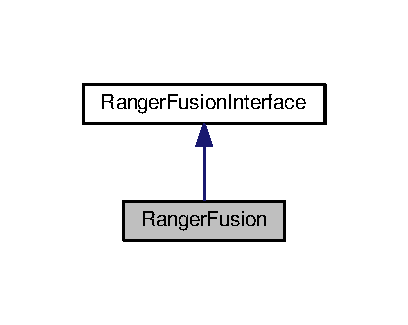
\includegraphics[width=196pt]{class_ranger_fusion__inherit__graph}
\end{center}
\end{figure}


Collaboration diagram for Ranger\+Fusion\+:
\nopagebreak
\begin{figure}[H]
\begin{center}
\leavevmode
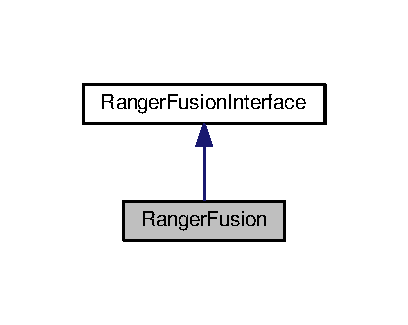
\includegraphics[width=196pt]{class_ranger_fusion__coll__graph}
\end{center}
\end{figure}
\subsection*{Classes}
\begin{DoxyCompactItemize}
\item 
struct \hyperlink{struct_ranger_fusion_1_1_point}{Point}
\begin{DoxyCompactList}\small\item\em Can be used to store cartesian 2D co-\/ordinates~\newline
. \end{DoxyCompactList}\end{DoxyCompactItemize}
\subsection*{Public Member Functions}
\begin{DoxyCompactItemize}
\item 
\hyperlink{class_ranger_fusion_a977f1817c88c33e8f35695a530e44a9c}{Ranger\+Fusion} (std\+::vector$<$ \hyperlink{class_ranger_interface}{Ranger\+Interface} $\ast$ $>$ rangers)
\item 
void \hyperlink{class_ranger_fusion_ae3128f8cc8f4cb955d8db661aefba3dc}{set\+Cells} (std\+::vector$<$ \hyperlink{class_cell}{Cell} $\ast$ $>$ cells)
\begin{DoxyCompactList}\small\item\em Accepts the container of cells. \end{DoxyCompactList}\item 
void \hyperlink{class_ranger_fusion_aa9265f72bc3572567c9cf98cf6d9f0e1}{grab\+And\+Fuse\+Data} ()\hypertarget{class_ranger_fusion_aa9265f72bc3572567c9cf98cf6d9f0e1}{}\label{class_ranger_fusion_aa9265f72bc3572567c9cf98cf6d9f0e1}

\begin{DoxyCompactList}\small\item\em Calls each ranger to generate data and combines range data with provided container of cells. Generates a \textquotesingle{}fusion\textquotesingle{} of the data based on collision conditions as descibed in Assignment 2 specification. \end{DoxyCompactList}\item 
std\+::vector$<$ std\+::vector$<$ double $>$ $>$ \hyperlink{class_ranger_fusion_a5780383fdffe121a7a2372a047819ba9}{get\+Raw\+Range\+Data} ()
\begin{DoxyCompactList}\small\item\em Returns the raw data from any sensors in the ranger container within a vector of vectors The raw data is updated every time a new fusion is requested. The raw data will match the preceeding fusion if it is called between fusions. If no fusion has occured the vector shall be empty. \end{DoxyCompactList}\item 
double \hyperlink{class_ranger_fusion_a7215e5405e808b5a853984e2b70ed6ad}{get\+Scanning\+Area} ()
\begin{DoxyCompactList}\small\item\em Returns the total scanning area possible with C\+O\+NE based scanners supplied. \end{DoxyCompactList}\item 
unsigned int \hyperlink{class_ranger_fusion_ad5f1752d3f1ddf1d4250c7e434971f1c}{get\+Sequence\+Number} (void)
\begin{DoxyCompactList}\small\item\em Returns sequence Number of Last fusion. \end{DoxyCompactList}\end{DoxyCompactItemize}


\subsection{Detailed Description}
\hyperlink{class_ranger_fusion}{Ranger\+Fusion} extract data from a collection of Rangers and fuses the data. . 

\subsection{Constructor \& Destructor Documentation}
\index{Ranger\+Fusion@{Ranger\+Fusion}!Ranger\+Fusion@{Ranger\+Fusion}}
\index{Ranger\+Fusion@{Ranger\+Fusion}!Ranger\+Fusion@{Ranger\+Fusion}}
\subsubsection[{\texorpdfstring{Ranger\+Fusion(std\+::vector$<$ Ranger\+Interface $\ast$ $>$ rangers)}{RangerFusion(std::vector< RangerInterface * > rangers)}}]{\setlength{\rightskip}{0pt plus 5cm}Ranger\+Fusion\+::\+Ranger\+Fusion (
\begin{DoxyParamCaption}
\item[{std\+::vector$<$ {\bf Ranger\+Interface} $\ast$ $>$}]{rangers}
\end{DoxyParamCaption}
)}\hypertarget{class_ranger_fusion_a977f1817c88c33e8f35695a530e44a9c}{}\label{class_ranger_fusion_a977f1817c88c33e8f35695a530e44a9c}
The Default constructor sets the cell centre to values within the \#\+M\+A\+P\+\_\+\+S\+I\+ZE~\newline
\begin{DoxySeeAlso}{See also}
\hyperlink{class_ranger_fusion_interface}{Ranger\+Fusion\+Interface} and 

\hyperlink{class_ranger_interface}{Ranger\+Interface} for more information 
\end{DoxySeeAlso}


\subsection{Member Function Documentation}
\index{Ranger\+Fusion@{Ranger\+Fusion}!get\+Raw\+Range\+Data@{get\+Raw\+Range\+Data}}
\index{get\+Raw\+Range\+Data@{get\+Raw\+Range\+Data}!Ranger\+Fusion@{Ranger\+Fusion}}
\subsubsection[{\texorpdfstring{get\+Raw\+Range\+Data()}{getRawRangeData()}}]{\setlength{\rightskip}{0pt plus 5cm}std\+::vector$<$ std\+::vector$<$ double $>$ $>$ Ranger\+Fusion\+::get\+Raw\+Range\+Data (
\begin{DoxyParamCaption}
{}
\end{DoxyParamCaption}
)\hspace{0.3cm}{\ttfamily [virtual]}}\hypertarget{class_ranger_fusion_a5780383fdffe121a7a2372a047819ba9}{}\label{class_ranger_fusion_a5780383fdffe121a7a2372a047819ba9}


Returns the raw data from any sensors in the ranger container within a vector of vectors The raw data is updated every time a new fusion is requested. The raw data will match the preceeding fusion if it is called between fusions. If no fusion has occured the vector shall be empty. 

\begin{DoxyReturn}{Returns}
std\+::vector$<$std\+::vector$<$double$>$$>$ the outer elements of the vector related to the rangers, the inner elements of vector the respective range readings 
\end{DoxyReturn}


Implements \hyperlink{class_ranger_fusion_interface_a9d60ca5866261026b870d7c0171587f5}{Ranger\+Fusion\+Interface}.

\index{Ranger\+Fusion@{Ranger\+Fusion}!get\+Scanning\+Area@{get\+Scanning\+Area}}
\index{get\+Scanning\+Area@{get\+Scanning\+Area}!Ranger\+Fusion@{Ranger\+Fusion}}
\subsubsection[{\texorpdfstring{get\+Scanning\+Area()}{getScanningArea()}}]{\setlength{\rightskip}{0pt plus 5cm}double Ranger\+Fusion\+::get\+Scanning\+Area (
\begin{DoxyParamCaption}
{}
\end{DoxyParamCaption}
)\hspace{0.3cm}{\ttfamily [virtual]}}\hypertarget{class_ranger_fusion_a7215e5405e808b5a853984e2b70ed6ad}{}\label{class_ranger_fusion_a7215e5405e808b5a853984e2b70ed6ad}


Returns the total scanning area possible with C\+O\+NE based scanners supplied. 

\begin{DoxyReturn}{Returns}
double Total area coverage 
\end{DoxyReturn}


Implements \hyperlink{class_ranger_fusion_interface_a65155605804376da4f67baf3c6f97f40}{Ranger\+Fusion\+Interface}.

\index{Ranger\+Fusion@{Ranger\+Fusion}!get\+Sequence\+Number@{get\+Sequence\+Number}}
\index{get\+Sequence\+Number@{get\+Sequence\+Number}!Ranger\+Fusion@{Ranger\+Fusion}}
\subsubsection[{\texorpdfstring{get\+Sequence\+Number(void)}{getSequenceNumber(void)}}]{\setlength{\rightskip}{0pt plus 5cm}unsigned int Ranger\+Fusion\+::get\+Sequence\+Number (
\begin{DoxyParamCaption}
\item[{void}]{}
\end{DoxyParamCaption}
)}\hypertarget{class_ranger_fusion_ad5f1752d3f1ddf1d4250c7e434971f1c}{}\label{class_ranger_fusion_ad5f1752d3f1ddf1d4250c7e434971f1c}


Returns sequence Number of Last fusion. 

\begin{DoxyReturn}{Returns}
unsigned int Sequence Number of Fusion 
\end{DoxyReturn}
\index{Ranger\+Fusion@{Ranger\+Fusion}!set\+Cells@{set\+Cells}}
\index{set\+Cells@{set\+Cells}!Ranger\+Fusion@{Ranger\+Fusion}}
\subsubsection[{\texorpdfstring{set\+Cells(std\+::vector$<$ Cell $\ast$ $>$ cells)}{setCells(std::vector< Cell * > cells)}}]{\setlength{\rightskip}{0pt plus 5cm}void Ranger\+Fusion\+::set\+Cells (
\begin{DoxyParamCaption}
\item[{std\+::vector$<$ {\bf Cell} $\ast$ $>$}]{cells}
\end{DoxyParamCaption}
)\hspace{0.3cm}{\ttfamily [virtual]}}\hypertarget{class_ranger_fusion_ae3128f8cc8f4cb955d8db661aefba3dc}{}\label{class_ranger_fusion_ae3128f8cc8f4cb955d8db661aefba3dc}


Accepts the container of cells. 


\begin{DoxyParams}{Parameters}
{\em cells} & \\
\hline
\end{DoxyParams}


Implements \hyperlink{class_ranger_fusion_interface_ab0b45c2c462124ce74d54eb226044beb}{Ranger\+Fusion\+Interface}.



The documentation for this class was generated from the following files\+:\begin{DoxyCompactItemize}
\item 
rangerfusion.\+h\item 
rangerfusion.\+cpp\end{DoxyCompactItemize}

\hypertarget{class_ranger_fusion_interface}{}\section{Ranger\+Fusion\+Interface Class Reference}
\label{class_ranger_fusion_interface}\index{Ranger\+Fusion\+Interface@{Ranger\+Fusion\+Interface}}


Specifies the required interface for your \hyperlink{class_ranger_fusion}{Ranger\+Fusion} class your ranger fusion class must inherit from it. {\bfseries  You M\+U\+ST N\+OT edit this file }.  




{\ttfamily \#include $<$rangerfusioninterface.\+h$>$}



Inheritance diagram for Ranger\+Fusion\+Interface\+:
\nopagebreak
\begin{figure}[H]
\begin{center}
\leavevmode
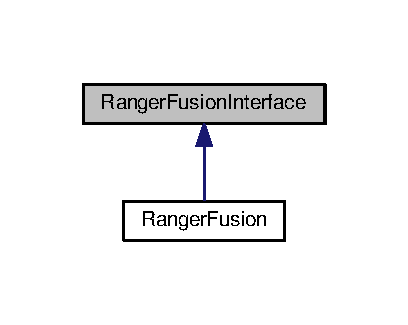
\includegraphics[width=196pt]{class_ranger_fusion_interface__inherit__graph}
\end{center}
\end{figure}
\subsection*{Public Member Functions}
\begin{DoxyCompactItemize}
\item 
virtual void \hyperlink{class_ranger_fusion_interface_ab0b45c2c462124ce74d54eb226044beb}{set\+Cells} (std\+::vector$<$ \hyperlink{class_cell}{Cell} $\ast$ $>$ cells)=0
\begin{DoxyCompactList}\small\item\em Accepts the container of cells. \end{DoxyCompactList}\item 
virtual void \hyperlink{class_ranger_fusion_interface_ada6afdab2ce6d58a1bd0134f5e2be23f}{grab\+And\+Fuse\+Data} ()=0\hypertarget{class_ranger_fusion_interface_ada6afdab2ce6d58a1bd0134f5e2be23f}{}\label{class_ranger_fusion_interface_ada6afdab2ce6d58a1bd0134f5e2be23f}

\begin{DoxyCompactList}\small\item\em Calls each ranger to generate data and combines range data with provided container of cells. Generates a \textquotesingle{}fusion\textquotesingle{} of the data based on collision conditions as descibed in Assignment 2 specification. \end{DoxyCompactList}\item 
virtual std\+::vector$<$ std\+::vector$<$ double $>$ $>$ \hyperlink{class_ranger_fusion_interface_a9d60ca5866261026b870d7c0171587f5}{get\+Raw\+Range\+Data} ()=0
\begin{DoxyCompactList}\small\item\em Returns the raw data from any sensors in the ranger container within a vector of vectors The raw data is updated every time a new fusion is requested. The raw data will match the preceeding fusion if it is called between fusions. If no fusion has occured the vector shall be empty. \end{DoxyCompactList}\item 
virtual double \hyperlink{class_ranger_fusion_interface_a65155605804376da4f67baf3c6f97f40}{get\+Scanning\+Area} ()=0
\begin{DoxyCompactList}\small\item\em Returns the total scanning area possible with C\+O\+NE based scanners supplied A union of all areas \href{https://en.wikipedia.org/wiki/Union_(set_theory)}{\tt https\+://en.\+wikipedia.\+org/wiki/\+Union\+\_\+(set\+\_\+theory)} \end{DoxyCompactList}\end{DoxyCompactItemize}


\subsection{Detailed Description}
Specifies the required interface for your \hyperlink{class_ranger_fusion}{Ranger\+Fusion} class your ranger fusion class must inherit from it. {\bfseries  You M\+U\+ST N\+OT edit this file }. 

\subsection{Member Function Documentation}
\index{Ranger\+Fusion\+Interface@{Ranger\+Fusion\+Interface}!get\+Raw\+Range\+Data@{get\+Raw\+Range\+Data}}
\index{get\+Raw\+Range\+Data@{get\+Raw\+Range\+Data}!Ranger\+Fusion\+Interface@{Ranger\+Fusion\+Interface}}
\subsubsection[{\texorpdfstring{get\+Raw\+Range\+Data()=0}{getRawRangeData()=0}}]{\setlength{\rightskip}{0pt plus 5cm}virtual std\+::vector$<$std\+::vector$<$double$>$ $>$ Ranger\+Fusion\+Interface\+::get\+Raw\+Range\+Data (
\begin{DoxyParamCaption}
{}
\end{DoxyParamCaption}
)\hspace{0.3cm}{\ttfamily [pure virtual]}}\hypertarget{class_ranger_fusion_interface_a9d60ca5866261026b870d7c0171587f5}{}\label{class_ranger_fusion_interface_a9d60ca5866261026b870d7c0171587f5}


Returns the raw data from any sensors in the ranger container within a vector of vectors The raw data is updated every time a new fusion is requested. The raw data will match the preceeding fusion if it is called between fusions. If no fusion has occured the vector shall be empty. 

\begin{DoxyReturn}{Returns}
std\+::vector$<$std\+::vector$<$double$>$$>$ the outer elements of the vector related to the rangers, the inner elements of vector the respective range readings
\end{DoxyReturn}
\begin{DoxySeeAlso}{See also}
\hyperlink{class_ranger_fusion_interface_ada6afdab2ce6d58a1bd0134f5e2be23f}{grab\+And\+Fuse\+Data} 
\end{DoxySeeAlso}


Implemented in \hyperlink{class_ranger_fusion_a5780383fdffe121a7a2372a047819ba9}{Ranger\+Fusion}.

\index{Ranger\+Fusion\+Interface@{Ranger\+Fusion\+Interface}!get\+Scanning\+Area@{get\+Scanning\+Area}}
\index{get\+Scanning\+Area@{get\+Scanning\+Area}!Ranger\+Fusion\+Interface@{Ranger\+Fusion\+Interface}}
\subsubsection[{\texorpdfstring{get\+Scanning\+Area()=0}{getScanningArea()=0}}]{\setlength{\rightskip}{0pt plus 5cm}virtual double Ranger\+Fusion\+Interface\+::get\+Scanning\+Area (
\begin{DoxyParamCaption}
{}
\end{DoxyParamCaption}
)\hspace{0.3cm}{\ttfamily [pure virtual]}}\hypertarget{class_ranger_fusion_interface_a65155605804376da4f67baf3c6f97f40}{}\label{class_ranger_fusion_interface_a65155605804376da4f67baf3c6f97f40}


Returns the total scanning area possible with C\+O\+NE based scanners supplied A union of all areas \href{https://en.wikipedia.org/wiki/Union_(set_theory)}{\tt https\+://en.\+wikipedia.\+org/wiki/\+Union\+\_\+(set\+\_\+theory)} 

\begin{DoxyReturn}{Returns}
double Total area coverage
\end{DoxyReturn}
\begin{DoxySeeAlso}{See also}
\hyperlink{class_ranger_fusion_interface_ada6afdab2ce6d58a1bd0134f5e2be23f}{grab\+And\+Fuse\+Data} 
\end{DoxySeeAlso}


Implemented in \hyperlink{class_ranger_fusion_a7215e5405e808b5a853984e2b70ed6ad}{Ranger\+Fusion}.

\index{Ranger\+Fusion\+Interface@{Ranger\+Fusion\+Interface}!set\+Cells@{set\+Cells}}
\index{set\+Cells@{set\+Cells}!Ranger\+Fusion\+Interface@{Ranger\+Fusion\+Interface}}
\subsubsection[{\texorpdfstring{set\+Cells(std\+::vector$<$ Cell $\ast$ $>$ cells)=0}{setCells(std::vector< Cell * > cells)=0}}]{\setlength{\rightskip}{0pt plus 5cm}virtual void Ranger\+Fusion\+Interface\+::set\+Cells (
\begin{DoxyParamCaption}
\item[{std\+::vector$<$ {\bf Cell} $\ast$ $>$}]{cells}
\end{DoxyParamCaption}
)\hspace{0.3cm}{\ttfamily [pure virtual]}}\hypertarget{class_ranger_fusion_interface_ab0b45c2c462124ce74d54eb226044beb}{}\label{class_ranger_fusion_interface_ab0b45c2c462124ce74d54eb226044beb}


Accepts the container of cells. 


\begin{DoxyParams}{Parameters}
{\em cells} & \\
\hline
\end{DoxyParams}


Implemented in \hyperlink{class_ranger_fusion_ae3128f8cc8f4cb955d8db661aefba3dc}{Ranger\+Fusion}.



The documentation for this class was generated from the following file\+:\begin{DoxyCompactItemize}
\item 
rangerfusioninterface.\+h\end{DoxyCompactItemize}

\hypertarget{class_ranger_interface}{}\section{Ranger\+Interface Class Reference}
\label{class_ranger_interface}\index{Ranger\+Interface@{Ranger\+Interface}}


Specifies the functionality for the \hyperlink{class_ranger}{Ranger} Class, your \hyperlink{class_ranger}{Ranger} class must inherit from it. {\bfseries  You M\+U\+ST N\+OT edit this file }.  




{\ttfamily \#include $<$rangerinterface.\+h$>$}



Inheritance diagram for Ranger\+Interface\+:
\nopagebreak
\begin{figure}[H]
\begin{center}
\leavevmode
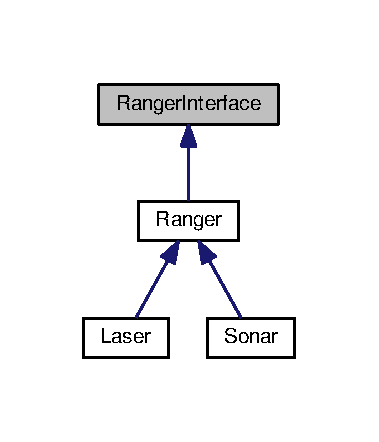
\includegraphics[width=182pt]{class_ranger_interface__inherit__graph}
\end{center}
\end{figure}
\subsection*{Public Member Functions}
\begin{DoxyCompactItemize}
\item 
virtual std\+::vector$<$ double $>$ {\bfseries generate\+Data} ()=0\hypertarget{class_ranger_interface_a969c670cadf55a15733809116dc305c8}{}\label{class_ranger_interface_a969c670cadf55a15733809116dc305c8}

\item 
virtual unsigned int \hyperlink{class_ranger_interface_a37d4f89daffa8b2708dfc11034893552}{get\+Angular\+Resolution} (void)=0
\item 
virtual int \hyperlink{class_ranger_interface_a3af867912dfc4f2cf899f53b82e85130}{get\+Angular\+Offset} (void)=0
\item 
virtual unsigned int \hyperlink{class_ranger_interface_a18716da6932402b8dda75f682be6f06c}{get\+Field\+Of\+View} (void)=0
\item 
virtual double \hyperlink{class_ranger_interface_a0bb29a41de5767c99081002c0590c186}{get\+Max\+Range} (void)=0
\item 
virtual double \hyperlink{class_ranger_interface_ae6d501ddeeaad4a7b44d7d51ce64cb88}{get\+Min\+Range} (void)=0
\item 
virtual ranger\+::\+Sensing\+Method \hyperlink{class_ranger_interface_aeb06b9835f2b162b81917bd27797549b}{get\+Sensing\+Method} (void)=0
\item 
virtual bool \hyperlink{class_ranger_interface_aecffc9bbb58379da741c18326b9e41db}{set\+Angular\+Resolution} (unsigned int resolution)=0
\item 
virtual bool \hyperlink{class_ranger_interface_a2ac537778d99306a378d151c544426dc}{set\+Angular\+Offset} (int offset)=0
\item 
virtual bool \hyperlink{class_ranger_interface_a70357ca516198af45e2d503ef6af8f9f}{set\+Field\+Of\+View} (unsigned int fov)=0
\end{DoxyCompactItemize}


\subsection{Detailed Description}
Specifies the functionality for the \hyperlink{class_ranger}{Ranger} Class, your \hyperlink{class_ranger}{Ranger} class must inherit from it. {\bfseries  You M\+U\+ST N\+OT edit this file }. 

\subsection{Member Function Documentation}
\index{Ranger\+Interface@{Ranger\+Interface}!get\+Angular\+Offset@{get\+Angular\+Offset}}
\index{get\+Angular\+Offset@{get\+Angular\+Offset}!Ranger\+Interface@{Ranger\+Interface}}
\subsubsection[{\texorpdfstring{get\+Angular\+Offset(void)=0}{getAngularOffset(void)=0}}]{\setlength{\rightskip}{0pt plus 5cm}virtual int Ranger\+Interface\+::get\+Angular\+Offset (
\begin{DoxyParamCaption}
\item[{void}]{}
\end{DoxyParamCaption}
)\hspace{0.3cm}{\ttfamily [pure virtual]}}\hypertarget{class_ranger_interface_a3af867912dfc4f2cf899f53b82e85130}{}\label{class_ranger_interface_a3af867912dfc4f2cf899f53b82e85130}
Getter for offset from Y axis \begin{DoxyReturn}{Returns}
angular resolution \mbox{[}deg\mbox{]} 
\end{DoxyReturn}


Implemented in \hyperlink{class_ranger_a1952b96d8dcbeb6afa107c8453d778a5}{Ranger}.

\index{Ranger\+Interface@{Ranger\+Interface}!get\+Angular\+Resolution@{get\+Angular\+Resolution}}
\index{get\+Angular\+Resolution@{get\+Angular\+Resolution}!Ranger\+Interface@{Ranger\+Interface}}
\subsubsection[{\texorpdfstring{get\+Angular\+Resolution(void)=0}{getAngularResolution(void)=0}}]{\setlength{\rightskip}{0pt plus 5cm}virtual unsigned int Ranger\+Interface\+::get\+Angular\+Resolution (
\begin{DoxyParamCaption}
\item[{void}]{}
\end{DoxyParamCaption}
)\hspace{0.3cm}{\ttfamily [pure virtual]}}\hypertarget{class_ranger_interface_a37d4f89daffa8b2708dfc11034893552}{}\label{class_ranger_interface_a37d4f89daffa8b2708dfc11034893552}
Getter for Angular resolution \begin{DoxyReturn}{Returns}
angular resolution \mbox{[}deg\mbox{]} 
\end{DoxyReturn}


Implemented in \hyperlink{class_ranger_a95b5013ae191d1e19b93fab002306718}{Ranger}.

\index{Ranger\+Interface@{Ranger\+Interface}!get\+Field\+Of\+View@{get\+Field\+Of\+View}}
\index{get\+Field\+Of\+View@{get\+Field\+Of\+View}!Ranger\+Interface@{Ranger\+Interface}}
\subsubsection[{\texorpdfstring{get\+Field\+Of\+View(void)=0}{getFieldOfView(void)=0}}]{\setlength{\rightskip}{0pt plus 5cm}virtual unsigned int Ranger\+Interface\+::get\+Field\+Of\+View (
\begin{DoxyParamCaption}
\item[{void}]{}
\end{DoxyParamCaption}
)\hspace{0.3cm}{\ttfamily [pure virtual]}}\hypertarget{class_ranger_interface_a18716da6932402b8dda75f682be6f06c}{}\label{class_ranger_interface_a18716da6932402b8dda75f682be6f06c}
Getter for field of view, for P\+O\+I\+NT based sensors F\+OV is zero \begin{DoxyReturn}{Returns}
field of view \mbox{[}deg\mbox{]} 
\end{DoxyReturn}


Implemented in \hyperlink{class_ranger_a4bca7dce56b7959257d90b1f30bf0271}{Ranger}.

\index{Ranger\+Interface@{Ranger\+Interface}!get\+Max\+Range@{get\+Max\+Range}}
\index{get\+Max\+Range@{get\+Max\+Range}!Ranger\+Interface@{Ranger\+Interface}}
\subsubsection[{\texorpdfstring{get\+Max\+Range(void)=0}{getMaxRange(void)=0}}]{\setlength{\rightskip}{0pt plus 5cm}virtual double Ranger\+Interface\+::get\+Max\+Range (
\begin{DoxyParamCaption}
\item[{void}]{}
\end{DoxyParamCaption}
)\hspace{0.3cm}{\ttfamily [pure virtual]}}\hypertarget{class_ranger_interface_a0bb29a41de5767c99081002c0590c186}{}\label{class_ranger_interface_a0bb29a41de5767c99081002c0590c186}
Getter for maximum range \begin{DoxyReturn}{Returns}
maximum rage \mbox{[}m\mbox{]} 
\end{DoxyReturn}


Implemented in \hyperlink{class_ranger_aba5e81260e55089d9ff869051156a722}{Ranger}.

\index{Ranger\+Interface@{Ranger\+Interface}!get\+Min\+Range@{get\+Min\+Range}}
\index{get\+Min\+Range@{get\+Min\+Range}!Ranger\+Interface@{Ranger\+Interface}}
\subsubsection[{\texorpdfstring{get\+Min\+Range(void)=0}{getMinRange(void)=0}}]{\setlength{\rightskip}{0pt plus 5cm}virtual double Ranger\+Interface\+::get\+Min\+Range (
\begin{DoxyParamCaption}
\item[{void}]{}
\end{DoxyParamCaption}
)\hspace{0.3cm}{\ttfamily [pure virtual]}}\hypertarget{class_ranger_interface_ae6d501ddeeaad4a7b44d7d51ce64cb88}{}\label{class_ranger_interface_ae6d501ddeeaad4a7b44d7d51ce64cb88}
Getter for mimimum range \begin{DoxyReturn}{Returns}
minimum rage \mbox{[}m\mbox{]} 
\end{DoxyReturn}


Implemented in \hyperlink{class_ranger_a646a06d3916179b9ebc4502bad169eec}{Ranger}.

\index{Ranger\+Interface@{Ranger\+Interface}!get\+Sensing\+Method@{get\+Sensing\+Method}}
\index{get\+Sensing\+Method@{get\+Sensing\+Method}!Ranger\+Interface@{Ranger\+Interface}}
\subsubsection[{\texorpdfstring{get\+Sensing\+Method(void)=0}{getSensingMethod(void)=0}}]{\setlength{\rightskip}{0pt plus 5cm}virtual ranger\+::\+Sensing\+Method Ranger\+Interface\+::get\+Sensing\+Method (
\begin{DoxyParamCaption}
\item[{void}]{}
\end{DoxyParamCaption}
)\hspace{0.3cm}{\ttfamily [pure virtual]}}\hypertarget{class_ranger_interface_aeb06b9835f2b162b81917bd27797549b}{}\label{class_ranger_interface_aeb06b9835f2b162b81917bd27797549b}
Getter for sensing method \begin{DoxyReturn}{Returns}
Sensing Method 
\end{DoxyReturn}
\begin{DoxySeeAlso}{See also}
Sensging Method 
\end{DoxySeeAlso}


Implemented in \hyperlink{class_ranger_a47e30b7ec55adec5bb542278ccfee140}{Ranger}.

\index{Ranger\+Interface@{Ranger\+Interface}!set\+Angular\+Offset@{set\+Angular\+Offset}}
\index{set\+Angular\+Offset@{set\+Angular\+Offset}!Ranger\+Interface@{Ranger\+Interface}}
\subsubsection[{\texorpdfstring{set\+Angular\+Offset(int offset)=0}{setAngularOffset(int offset)=0}}]{\setlength{\rightskip}{0pt plus 5cm}virtual bool Ranger\+Interface\+::set\+Angular\+Offset (
\begin{DoxyParamCaption}
\item[{int}]{offset}
\end{DoxyParamCaption}
)\hspace{0.3cm}{\ttfamily [pure virtual]}}\hypertarget{class_ranger_interface_a2ac537778d99306a378d151c544426dc}{}\label{class_ranger_interface_a2ac537778d99306a378d151c544426dc}
Set angular offset 
\begin{DoxyParams}{Parameters}
{\em offset} & \mbox{[}degrees\mbox{]} \\
\hline
\end{DoxyParams}
\begin{DoxyReturn}{Returns}
true if offset actioned, false otherwise 
\end{DoxyReturn}


Implemented in \hyperlink{class_ranger_ae1b15546cf48d942f86ea1031e9be486}{Ranger}.

\index{Ranger\+Interface@{Ranger\+Interface}!set\+Angular\+Resolution@{set\+Angular\+Resolution}}
\index{set\+Angular\+Resolution@{set\+Angular\+Resolution}!Ranger\+Interface@{Ranger\+Interface}}
\subsubsection[{\texorpdfstring{set\+Angular\+Resolution(unsigned int resolution)=0}{setAngularResolution(unsigned int resolution)=0}}]{\setlength{\rightskip}{0pt plus 5cm}virtual bool Ranger\+Interface\+::set\+Angular\+Resolution (
\begin{DoxyParamCaption}
\item[{unsigned int}]{resolution}
\end{DoxyParamCaption}
)\hspace{0.3cm}{\ttfamily [pure virtual]}}\hypertarget{class_ranger_interface_aecffc9bbb58379da741c18326b9e41db}{}\label{class_ranger_interface_aecffc9bbb58379da741c18326b9e41db}
Set angular resolution method 
\begin{DoxyParams}{Parameters}
{\em resolution} & in \mbox{[}degrees\mbox{]} \\
\hline
\end{DoxyParams}
\begin{DoxyReturn}{Returns}
true if resolution supported and actioned, false is not -\/ previous setting used 
\end{DoxyReturn}


Implemented in \hyperlink{class_ranger_a3dc62dcba54eefbd7a0f08cbf97d87dc}{Ranger}.

\index{Ranger\+Interface@{Ranger\+Interface}!set\+Field\+Of\+View@{set\+Field\+Of\+View}}
\index{set\+Field\+Of\+View@{set\+Field\+Of\+View}!Ranger\+Interface@{Ranger\+Interface}}
\subsubsection[{\texorpdfstring{set\+Field\+Of\+View(unsigned int fov)=0}{setFieldOfView(unsigned int fov)=0}}]{\setlength{\rightskip}{0pt plus 5cm}virtual bool Ranger\+Interface\+::set\+Field\+Of\+View (
\begin{DoxyParamCaption}
\item[{unsigned int}]{fov}
\end{DoxyParamCaption}
)\hspace{0.3cm}{\ttfamily [pure virtual]}}\hypertarget{class_ranger_interface_a70357ca516198af45e2d503ef6af8f9f}{}\label{class_ranger_interface_a70357ca516198af45e2d503ef6af8f9f}
Set field of view 
\begin{DoxyParams}{Parameters}
{\em field} & of view \mbox{[}degrees\mbox{]} \\
\hline
\end{DoxyParams}
\begin{DoxyReturn}{Returns}
true if field of view actioned, false otherwise 
\end{DoxyReturn}


Implemented in \hyperlink{class_ranger_a9cebe84c1aec338dc0b72baff48ea9d4}{Ranger}, \hyperlink{class_laser_a5f140784aae7e82c2aa0f690548d6ebb}{Laser}, and \hyperlink{class_sonar_a74d551d0ad61861ccf903f2535d799f0}{Sonar}.



The documentation for this class was generated from the following file\+:\begin{DoxyCompactItemize}
\item 
rangerinterface.\+h\end{DoxyCompactItemize}

\hypertarget{class_sonar}{}\section{Sonar Class Reference}
\label{class_sonar}\index{Sonar@{Sonar}}


\hyperlink{class_sonar}{Sonar} Shoots one broad sonar that covers its field of view and returns maximum distance it reached.  




{\ttfamily \#include $<$sonar.\+h$>$}



Inheritance diagram for Sonar\+:
\nopagebreak
\begin{figure}[H]
\begin{center}
\leavevmode
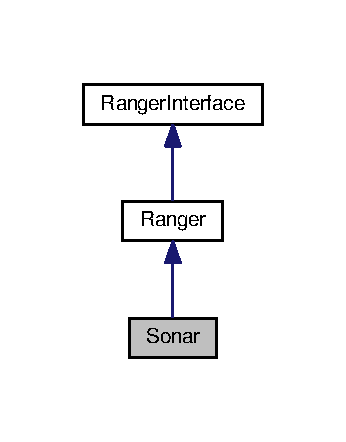
\includegraphics[width=166pt]{class_sonar__inherit__graph}
\end{center}
\end{figure}


Collaboration diagram for Sonar\+:
\nopagebreak
\begin{figure}[H]
\begin{center}
\leavevmode
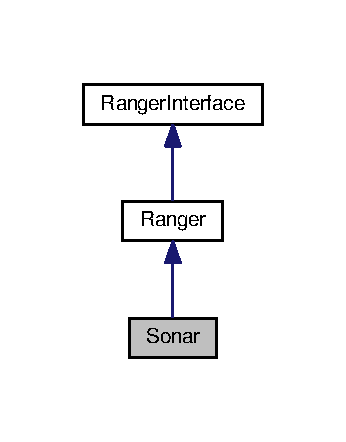
\includegraphics[width=166pt]{class_sonar__coll__graph}
\end{center}
\end{figure}
\subsection*{Public Member Functions}
\begin{DoxyCompactItemize}
\item 
\hyperlink{class_sonar_a71ef009d138f1e372fc35ca0cb6e85e2}{Sonar} ()
\item 
bool \hyperlink{class_sonar_a74d551d0ad61861ccf903f2535d799f0}{set\+Field\+Of\+View} (unsigned int fov)
\item 
std\+::vector$<$ double $>$ \hyperlink{class_sonar_a33cc5f2df6cc1d96a59067be67eab781}{generate\+Data} ()
\begin{DoxyCompactList}\small\item\em This function generates random range readings as data using supplied random number generator~\newline
using normal distribution with mean of 4m and standard deviation of 5m. \end{DoxyCompactList}\item 
\hyperlink{struct_ranger_1_1data_sequence_num}{data\+Sequence\+Num} \hyperlink{class_sonar_a962c7ba3b9a69e6b3b285764dd4eec3c}{query\+Sample} (unsigned int \&a)
\end{DoxyCompactItemize}
\subsection*{Additional Inherited Members}


\subsection{Detailed Description}
\hyperlink{class_sonar}{Sonar} Shoots one broad sonar that covers its field of view and returns maximum distance it reached. 

The \hyperlink{class_sonar}{Sonar} works accordingly\+: ~\newline
It shoots a broad cone shaped sonar wave that covers field of view completely.~\newline
Then it returns the maximum distance the sonar reaches.~\newline
 

\subsection{Constructor \& Destructor Documentation}
\index{Sonar@{Sonar}!Sonar@{Sonar}}
\index{Sonar@{Sonar}!Sonar@{Sonar}}
\subsubsection[{\texorpdfstring{Sonar()}{Sonar()}}]{\setlength{\rightskip}{0pt plus 5cm}Sonar\+::\+Sonar (
\begin{DoxyParamCaption}
{}
\end{DoxyParamCaption}
)}\hypertarget{class_sonar_a71ef009d138f1e372fc35ca0cb6e85e2}{}\label{class_sonar_a71ef009d138f1e372fc35ca0cb6e85e2}
Default constructor -\/ all sensor attributes set to a default values for \hyperlink{class_sonar}{Sonar} 

\subsection{Member Function Documentation}
\index{Sonar@{Sonar}!generate\+Data@{generate\+Data}}
\index{generate\+Data@{generate\+Data}!Sonar@{Sonar}}
\subsubsection[{\texorpdfstring{generate\+Data()}{generateData()}}]{\setlength{\rightskip}{0pt plus 5cm}std\+::vector$<$ double $>$ Sonar\+::generate\+Data (
\begin{DoxyParamCaption}
{}
\end{DoxyParamCaption}
)\hspace{0.3cm}{\ttfamily [virtual]}}\hypertarget{class_sonar_a33cc5f2df6cc1d96a59067be67eab781}{}\label{class_sonar_a33cc5f2df6cc1d96a59067be67eab781}


This function generates random range readings as data using supplied random number generator~\newline
using normal distribution with mean of 4m and standard deviation of 5m. 

Member function to generate range reading for \hyperlink{class_sonar}{Sonar} \begin{DoxyReturn}{Returns}
dataset of range reading of \hyperlink{class_sonar}{Sonar}\mbox{[}m\mbox{]} 
\end{DoxyReturn}


Implements \hyperlink{class_ranger_a1ac4a84f251b0793fc262643080f084a}{Ranger}.

\index{Sonar@{Sonar}!query\+Sample@{query\+Sample}}
\index{query\+Sample@{query\+Sample}!Sonar@{Sonar}}
\subsubsection[{\texorpdfstring{query\+Sample(unsigned int \&a)}{querySample(unsigned int &a)}}]{\setlength{\rightskip}{0pt plus 5cm}{\bf Sonar\+::data\+Sequence\+Num} Sonar\+::query\+Sample (
\begin{DoxyParamCaption}
\item[{unsigned int \&}]{a}
\end{DoxyParamCaption}
)\hspace{0.3cm}{\ttfamily [virtual]}}\hypertarget{class_sonar_a962c7ba3b9a69e6b3b285764dd4eec3c}{}\label{class_sonar_a962c7ba3b9a69e6b3b285764dd4eec3c}
Member function that can be used to query stored data of \hyperlink{class_sonar}{Sonar} 
\begin{DoxyParams}{Parameters}
{\em Desired} & Sample Number \\
\hline
\end{DoxyParams}
\begin{DoxyReturn}{Returns}
a struct that consists of\+: ~\newline

\begin{DoxyItemize}
\item Sample Number~\newline

\item Dataset\mbox{[}m\mbox{]} 
\end{DoxyItemize}
\end{DoxyReturn}


Implements \hyperlink{class_ranger_adbde91455d069a471c890e2aa808c0d3}{Ranger}.

\index{Sonar@{Sonar}!set\+Field\+Of\+View@{set\+Field\+Of\+View}}
\index{set\+Field\+Of\+View@{set\+Field\+Of\+View}!Sonar@{Sonar}}
\subsubsection[{\texorpdfstring{set\+Field\+Of\+View(unsigned int fov)}{setFieldOfView(unsigned int fov)}}]{\setlength{\rightskip}{0pt plus 5cm}bool Sonar\+::set\+Field\+Of\+View (
\begin{DoxyParamCaption}
\item[{unsigned int}]{fov}
\end{DoxyParamCaption}
)\hspace{0.3cm}{\ttfamily [virtual]}}\hypertarget{class_sonar_a74d551d0ad61861ccf903f2535d799f0}{}\label{class_sonar_a74d551d0ad61861ccf903f2535d799f0}
Member function sets Field of View 
\begin{DoxyParams}{Parameters}
{\em Desired} & Field of View \\
\hline
\end{DoxyParams}
\begin{DoxyReturn}{Returns}
a boolean indicating if passed value is compatible with \hyperlink{class_sonar}{Sonar}. 
\end{DoxyReturn}


Implements \hyperlink{class_ranger_a9cebe84c1aec338dc0b72baff48ea9d4}{Ranger}.



The documentation for this class was generated from the following files\+:\begin{DoxyCompactItemize}
\item 
sonar.\+h\item 
sonar.\+cpp\end{DoxyCompactItemize}

%--- End generated contents ---

% Index
\backmatter
\newpage
\phantomsection
\clearemptydoublepage
\addcontentsline{toc}{chapter}{Index}
\printindex

\end{document}
